\chapter{Proof-of-Concept Applicatie}
\label{ch:ontwikkeling}

\section{Inleiding}

Dit hoofdstuk dient als een uitgebreide toelichting op de softwareoplossing die binnen deze bachelorproef is ontwikkeld.
Eerst zal de algemene architectuur van de applicatie worden besproken, gevolgd door een gedetailleerde uitleg van de verschillende componenten.
Aangezien er rekening gehouden werd met het effectief inzetten van de applicatie in de praktijk, zullen ook de gebruikte Technologieën en technische keuzes worden toegelicht.
Zo kan de software voor opeenvolgende bachelorproeven iteratief verder ontwikkeld worden naar nieuwe functionaliteiten en verbeteringen.

\section{Architectuur}

De workflow die werd bedacht voor de proof-of-concept applicatie, om van ruwe data naar bruikbare metrieken te gaan, kan als volgt worden samengevat:
\begin{enumerate}
    \item Er worden één of meerdere `kalibratie-opnames` gemaakt met de eyetrackingbril, waarbij elk object waar men geïnteresseerd in is vanuit verschillende hoeken wordt gefilmd.
    \item Ook worden er opnames gemaakt die geanalyseerd dienen te worden, waarbij de studenten in de simulatieomgeving met de eyetrackingbril rondlopen.
    \item De opnames worden geïmporteerd in de applicatie via de WiFi-verbinding van de eyetrackingbril.
    \item Men geeft een naam aan de simulatieomgeving (bijvoorbeeld `Zorglab Zorgkamer`) binnen de applicatie en defininieert de objecten.
    \item Daarna kan men beginnen met het labelen van de objecten in de kalibratie-opnames via de ingebouwde labeling-tool. Dit dient als een basis voor het trainen of initialiseren van de analysemodellen.
    \item De applicatie is nu in staat de eyetracking-opnames van de studenten te analyseren en de metrieken te visualiseren. Dit deel werd niet verder uitgewerkt binnen deze bachelorproef omdat er niet tot een betrouwbaar analysemodel kon worden gekomen, maar verder hierover in Hoofdstuk~\ref{ch:experiment}.
\end{enumerate}
De applicatie is dus opgebouwd uit verschillende componenten die samen een stapsgewijs proces vormen. Deze zullen hieronder verder worden toegelicht.

\subsection{Opnames Maken}

% TODO

\subsection{Importeren van Eyetracking-Opnames}

Zoals eerder vermeld heeft de Tobii eyetracker twee componenten: de bril zelf en een `hub`' die stroom levert aan de bril en de opnames opslaat op een SD-kaart.
Het zou dus mogelijk zijn om de opnames via de SD-kaart te importeren, maar dit is niet praktisch omdat de SD-kaart steeds uit de hub dient gehaald te worden.
Daarom biedt de hub ook een WiFi-verbinding aan, zodat de opnames via een netwerkverbinding kunnen worden geïmporteerd. 

Wanneer men de applicatie opent op de pagina `Browse Recordings` via de navigatiekolom, worden er twee tabellen getoond (zie figuur \ref{fig:browse-recordings}): de bovenstaande tabel `Local Recordings` toont de opnames die lokaal zijn opgeslagen op de computer, en de onderste tabel `Recordings on Tobii Glasses` toont de opnames die zijn opgeslagen op de hub.
Indien een tabel geen opnames bevat, wordt er een passend bericht getoond.
De opnames worden getoond in tabellen met de naam van de opname, de datum en tijd waarop deze werd gemaakt, en de duur van de opname. 
Het is mogelijk om opnames te verwijderen uit de `Local Recordings`-tabel door op de rode knop met het prullenbakje te klikken binnen de rij van een opname. Dit heeft geen invloed op de opnames die zijn opgeslagen op de hub.
Ook kan men zoeken naar opnames via de zoekbalk bovenaan de tabellen, en sorteren op naam, datum of duur door op de bijhorende kolomkop te klikken.

Wanneer de bril niet verbonden is met de computer, wordt er een bijhorende melding getoond, met een knop om opnieuw te verbinden. Figuur \ref{fig:browse-recordings} toont een voorbeeld van de interface van de applicatie, waar de bril niet verbonden is met de computer.
Linksonder in de interface toont de applicatie de huidige status van de verbinding met de bril, inclusief de batterijstatus. Bij figuur \ref{fig:browse-recordings-connected} is de bril wel verbonden met de computer. 
Elke rij in de onderste tabel bevat een blauwe knop met een pijl naar beneden, waarmee een opname kan worden geïmporteerd van de bril naar de computer. Dit kan enige tijd duren, afhankelijk van de grootte van de opname.

\begin{figure}[H]
  \centering
  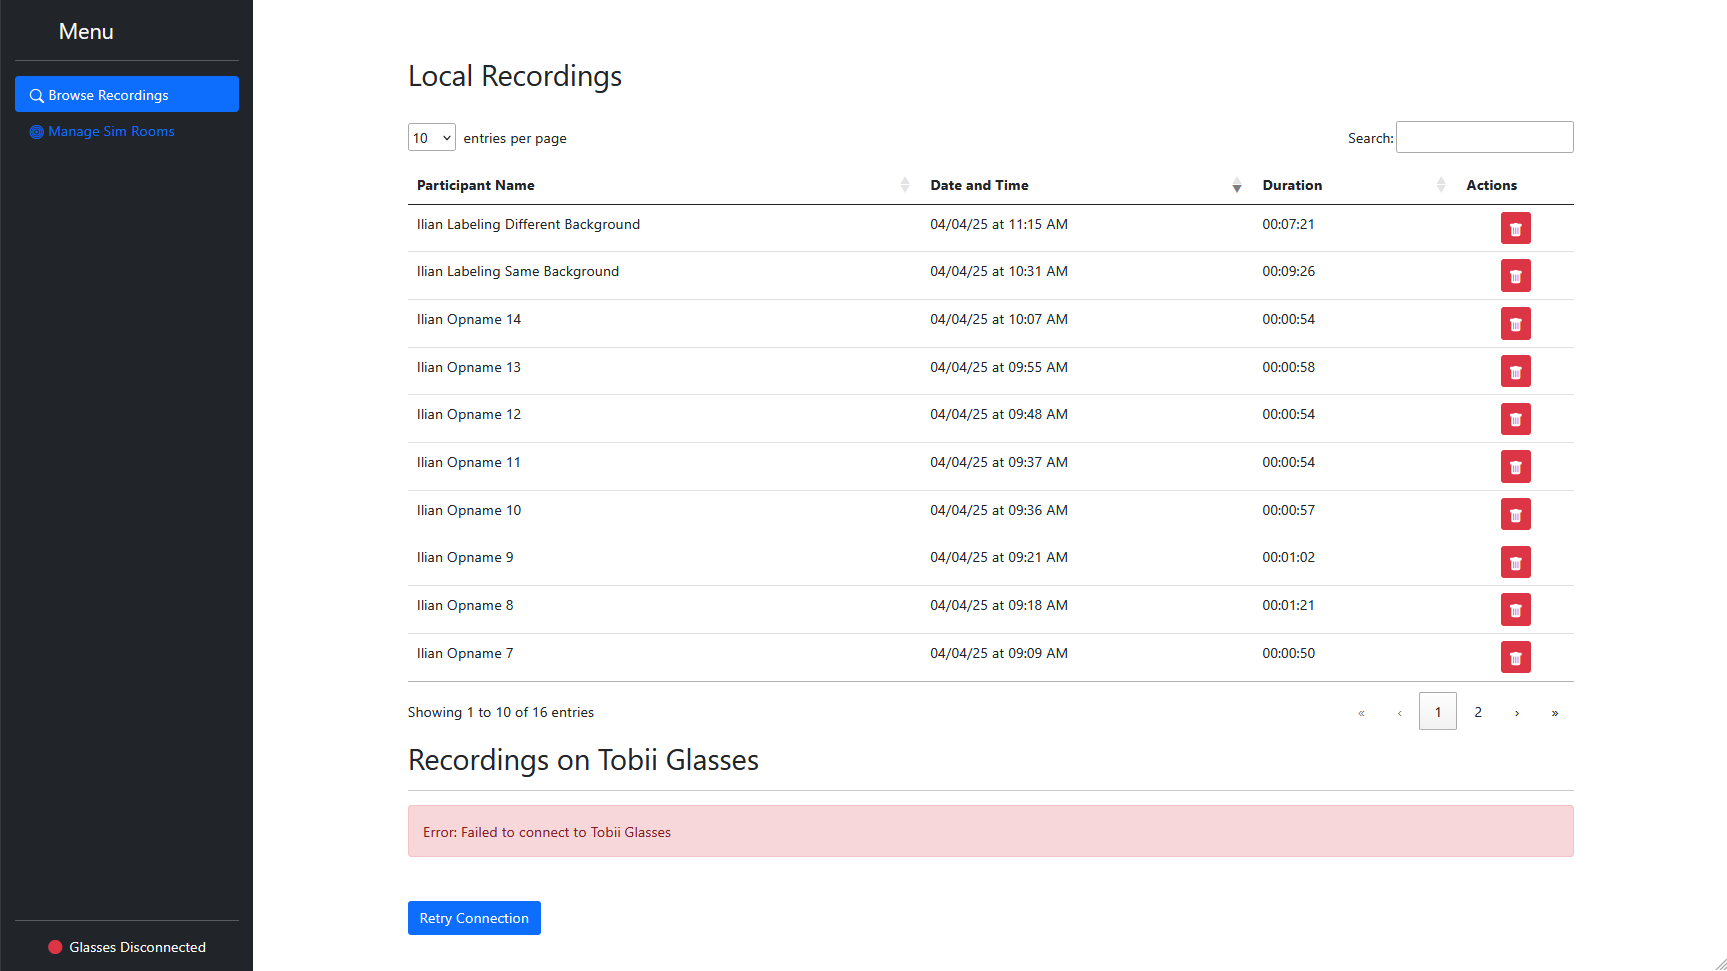
\includegraphics[width=1\textwidth]{browse-recordings.png}
  \caption[]{\label{fig:browse-recordings} Interface van de applicatie waar de opnames kunnen worden geïmporteerd. Hier is de bril niet verbonden met de computer. }
\end{figure}

\begin{figure}[H]
  \centering
  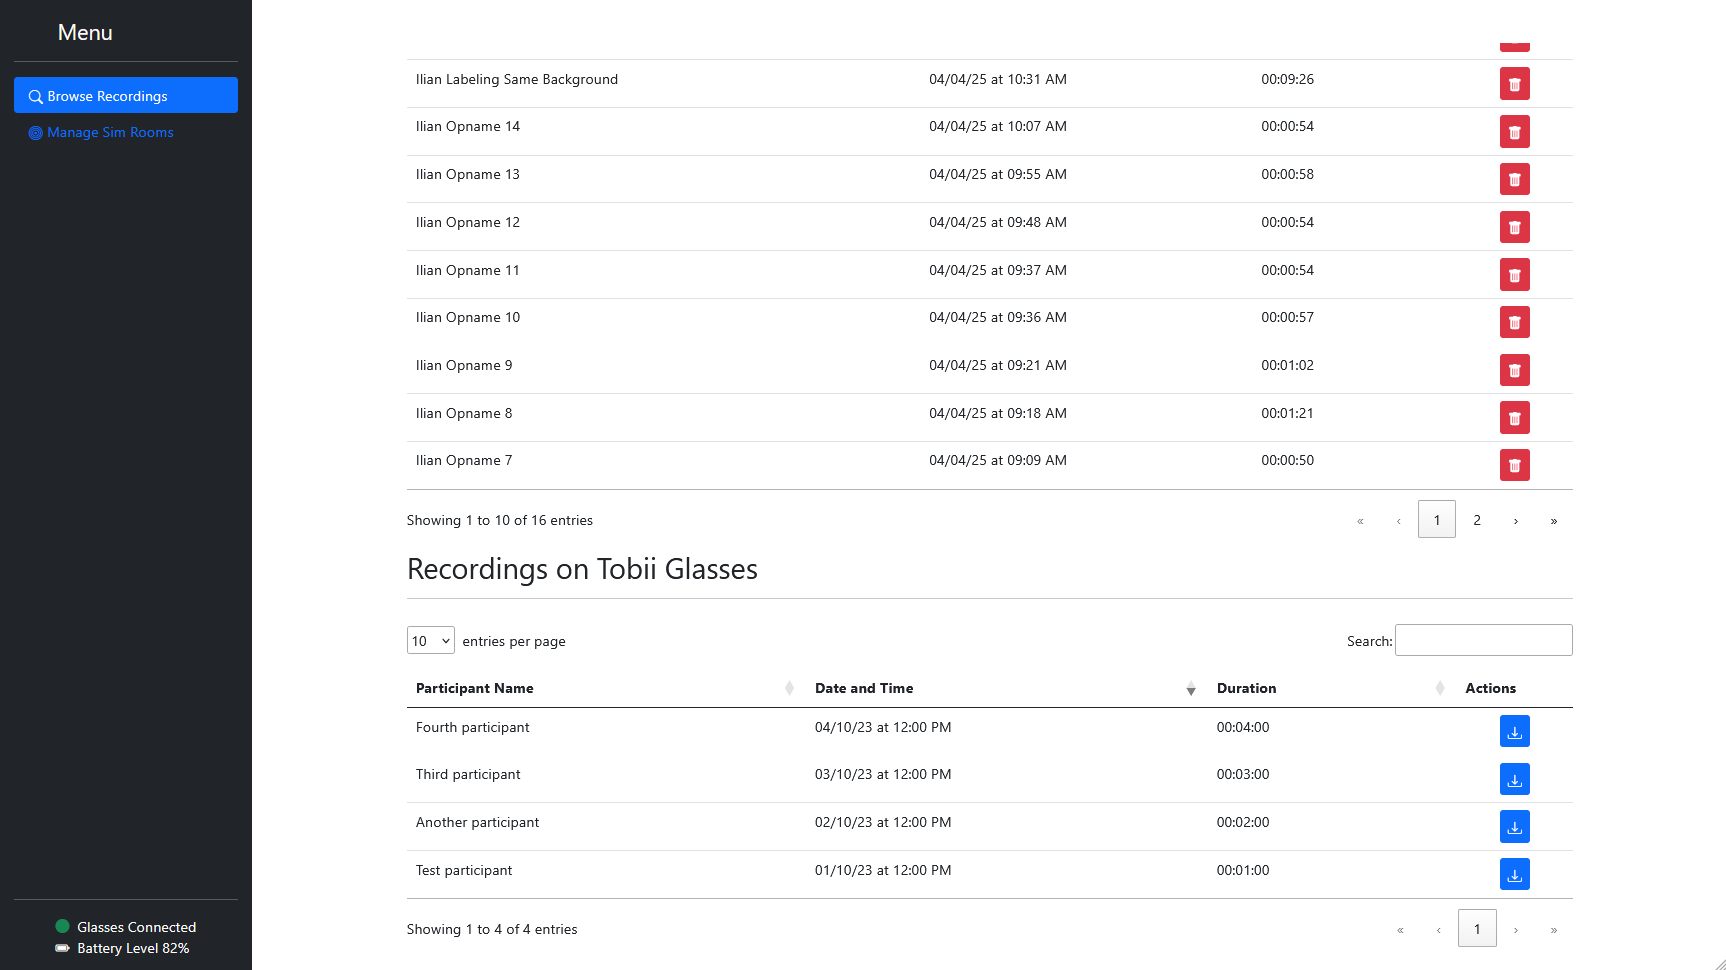
\includegraphics[width=1\textwidth]{browse-recordings-connected.png}
  \caption[]{\label{fig:browse-recordings-connected} Bij dit voorbeeld is de bril wel verbonden met de computer. Men ziet linksonder de batterlijstatus van de bril. In de onderste tabel is het mogelijk om opnames te importeren van de bril naar de computer. }
\end{figure}

\subsection{Simulatieruimten en Objecten}

Eens de opnames zijn geïmporteerd, kunnen we overgaan tot het labelen van de objecten in de kalibratie-opnames. Één van de design-keuzes was om met zogenaamde `simulatieruimten` te werken, die verschillende omgevingen voorstellen met elk hun eigen objecten.
Men kan zich dus voorstellen dat men niet enkel in het Zorglab werkt, maar bijvoorbeeld ook in een echt ziekenhuis of een woonzorgcentrum. Het doel was dus om de applicatie generiek mogelijk te maken, om het werk van de trainers te vergemakkelijken.

\begin{figure}[H]
  \centering
  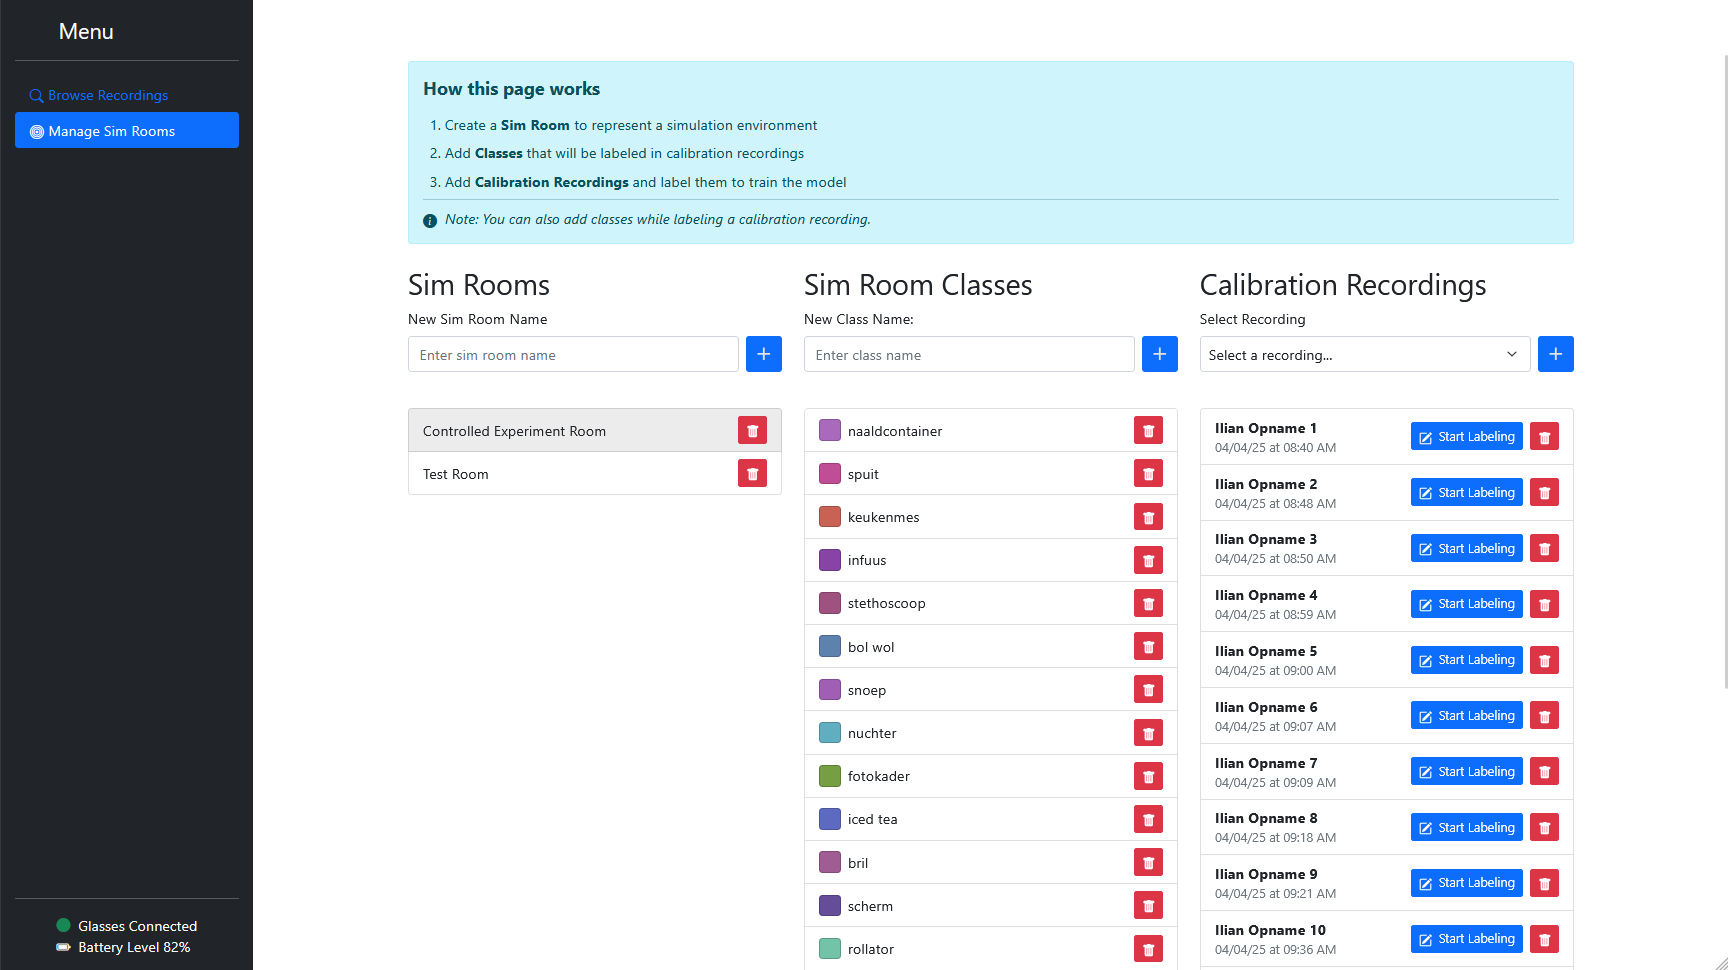
\includegraphics[width=1\textwidth]{simrooms.png}
  \caption[]{\label{fig:simrooms} Voorbeeld van de interface waar de simulatieomgevingen kunnen worden gedefinieerd. Hier is de `Controlled Experiment Room` geselecteerd, met een aantal objecten en kalibratie-opnames. }
\end{figure}

In figuur \ref{fig:simrooms} is een voorbeeld te zien van de interface waar simulatieomgevingen kunnen worden gedefinieerd. 
Deze interface heeft drie kolommen:
\begin{itemize}
    \item De eerste kolom toont de reeds gedefinieerde simulatieomgevingen, met hun naam, een knop om deze te verwijderen, en een invoerveld om een simulatieomgeving toe te voegen.
    \item Wanneer een simulatieomgeving is geselecteerd, worden de bijhorende objecten getoond in de tweede kolom. Elk object krijgt automatisch een kleur toegewezen dat ook gebruikt zal worden in de labeling-tool, en de visualisatie van de metrieken.
    \item In de derde kolom kan men geïmporteerde opnames selecteren om deze te gebruiken als kalibratie-opnames. Elke kalibratie-opname heeft een knop "Start Labeling"; wanneer men hierop klikt, wordt de labeling-tool geopend met de geselecteerde opname.
\end{itemize}

Merk op dat het mogelijk is om welke opname dan ook te selecteren als kalibratie-opname, waardoor ook praktijkopnames kunnen worden gebruikt!
Zo kunnen reeds gemaakte opnames van studenten ook worden gebruikt om de applicatie te trainen.
Ook stelt dit de applicatie eventueel in staat om de opnames te analyseren op basis van manuele annotaties van de trainers.
Deze aanpak zal meer tijd kosten, maar is veel nauwkeuriger dan automatische analyse. Aangezien het in deze bachelorproef gaat om geautomatiseerde analyse, werd deze optie niet verder uitgewerkt.

Wanneer men een kalibratie-opname verwijdert, heeft dit geen invloed op de opname zelf, maar enkel op de associatie met de simulatieomgeving.
Indien er met de opname werd gelabeld binnen deze simulatieomgeving, worden deze annotaties wel verwijderd. 
Hetzelfde geldt voor de objecten: indien een object wordt verwijderd, worden ook de annotaties met dat object verwijderd.

\subsection{Labeling Tool}

We hebben het al eerder gehad over de labeling-tool, maar hoe werkt deze nu precies? Dit is een van de belangrijkste onderdelen van de applicatie, en ook de meest complexe.

\subsection{Analyse van Eyetracking-Opnames}

\section{Operationele Prestaties}

\section{Gebruikte Technologieën}